\newpage
\section{Systeem niveau}
\label{Systeem_niveau}
De applicatie wordt gerepresenteerd als een black box. Dit is weergegeven in Figuur \ref{black_box} met de specificatie weergegeven in Tabel \ref{tab:Systeem_black_box}.
\\
\newline
\begin{figure}[H]
    \centering
    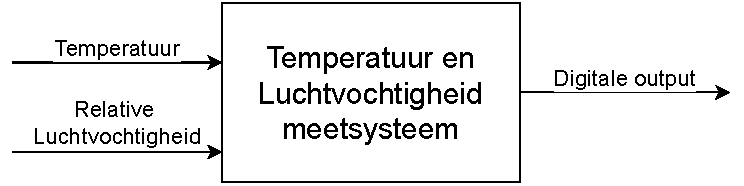
\includegraphics[width=0.8\linewidth]{pictures/Systeem_niveau_Systeemontwerp.drawio.pdf}
    \caption{Systeem ontwerp}
    \label{black_box}
\end{figure}
\begin{table}[H]
    \centering
    \caption{Specificaties op systeemontwerpniveau.}
    \begin{tabular}{|c|c|}
        \hline
        \textbf{Module}      & \textbf{Temperatuur en Luchtvochtigheid meetsysteem} \\ 
        \hline
        \textbf{Ingangen}    & \begin{tabular}[c]{@{}c@{}}  
        Temperatuur: -5 - 55 $^\circ\text{C}$ met 0,1 $^\circ\text{C}$ nauwkeurigheid \\ 
        Relatieve luchtvochtigheid: 0,1 - 100 \% met 2 \% nauwkeurigheid \\
        \end{tabular} \\
        \hline
        \textbf{Digitale uitgang(en)} & \begin{tabular}[c]{@{}c@{}} 
        Temperatuur: in bits \\
        Relatieve luchtvochtigheid: in bits \\
        Absolute luchtvochtigheid: in bits \\
        \end{tabular} \\
        \hline
        \textbf{Functie} & \begin{tabular}[c]{@{}c@{}} 
        Berekent de relatieve luchtvochtigheid. \\
        De informatie moet draadloos verstuurd worden naar het basisstation. \\
        Het meetsysteem moet vanuit batterijen gevoed worden. \end{tabular} \\ \hline
    \end{tabular}
    \label{tab:Systeem_black_box}
\end{table}

Uit dit black box schema ontstaan de volgende subsystemen. Het eerste subsysteem is de temperatuur sensor die de temperatuur meet uit de omgeving. En dit omzetten naar een elektronische grootheid zoals is weergegeven in Figuur \ref{fig:temper_systeemontwerp_temp} en Tabel \ref{tab:systeem_temper_sub_system}. Dit subsysteem is niet mogelijk om uit te zetten, omdat anders de metingen inaccuraat worden. 
\begin{figure}[H]
    \centering
    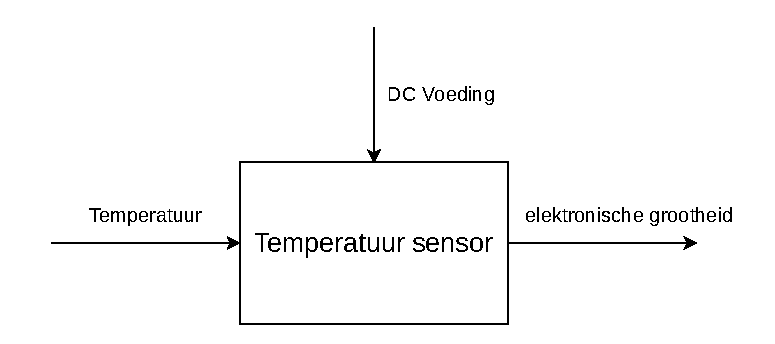
\includegraphics[width=0.45\linewidth]{pictures/Systeem_niveau_Systeemontwerp_temperatuur_sensor.drawio.pdf}
    \caption{Temperatuur sensor subsysteem.}
    \label{fig:temper_systeemontwerp_temp}
\end{figure}
\begin{table}[H]
    \centering
    \caption{Specificaties van Temperatuur sensor subsysteem}
    \begin{tabular}{|c|c|}
        \hline
        \textbf{Module} & \textbf{Temperatuur Sensor} \\
        \hline
        \textbf{Ingangen} &  \begin{tabular}[c]{@{}c@{}}
        Temperatuur: -5 - 55 $^\circ\text{C}$ met 0,1 $^\circ\text{C}$ nauwkeurigheid \\
        DC-voeding \\
        \end{tabular} \\
        \hline
        \textbf{Uitgang(en)} & Temperatuur sensor uitgang: ? elektronische grootheid \\
        \hline
        \textbf{Functie} & \begin{tabular}[c]{@{}c@{}}
        Meet de Temperatuur in de omgeving en \\
        vormt dit om naar een elektronische grootheid. \\
        \end{tabular} \\
        \hline
    \end{tabular}
    \label{tab:systeem_temper_sub_system}
\end{table}

Het tweede subsysteem is de relatieve luchtvochtigheid sensor. Dit subsysteem zet de relatieve luchtvochtigheid uit de omgeving om naar een binaire waarde. Deze waarde kan dan met een data protocol uitgelezen worden. Deze informatie moet dan door een digitaal systeem verwerkt worden, zodat het door de volgende subsystemen in het systeem gebruikt kan worden. Doordat dit subsysteem digitaal werkt, is het mogelijk om het systeem in rust stand of zelfs uit te zetten. Dit kan ervoor zorgen dat de energie van het subsysteem naar benenden gaat en er door andere subsystemen meer vermogen gebruikt kan worden. Het subsysteem is weergegeven in Figuur \ref{fig:systeem_relative_hum_sub_system} en Tabel \ref{tab:systeem_rel_hum_sub_system}.

\begin{figure}[H]
    \centering
    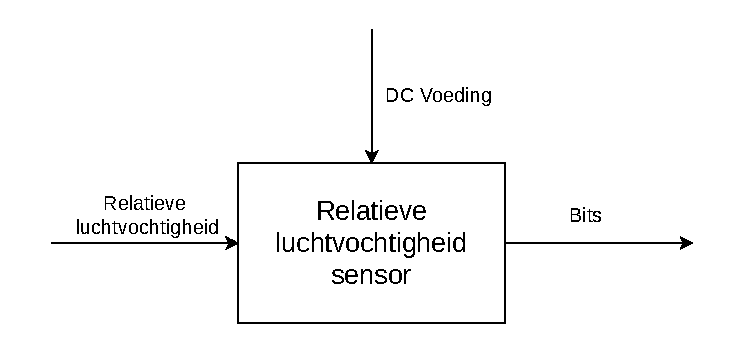
\includegraphics[width=0.45\linewidth]{pictures/Systeem_niveau_Systeemontwerp_relatieve_luchtvochtigheid.drawio.pdf}
    \caption{Relatieve luchtvochtigheid subsysteem.}
    \label{fig:systeem_relative_hum_sub_system}
\end{figure}
\begin{table}[H]
    \centering
    \caption{Specificaties van Relatieve luchtvochtigheid sensor subsysteem}
    \begin{tabular}{|c|c|}
        \hline
        \textbf{Module} & \textbf{Relatieve luchtvochtigheid Sensor} \\
        \hline
        \textbf{Ingangen} &  \begin{tabular}[c]{@{}c@{}}
        Relatieve luchtvochtigheid: 0,1 - 100 \% met 2 \% nauwkeurigheid \\
        DC-voeding \\
        \end{tabular} \\
        \hline
        \textbf{Uitgang(en)} & Relatieve luchtvochtigheid sensor uitgang: Bits \\
        \hline
        \textbf{Functie} & \begin{tabular}[c]{@{}c@{}}
        Meet de Relatieve luchtvochtigheid in de omgeving en \\
        vormt dit om naar een binaire waarde. \\
        \end{tabular} \\
        \hline
    \end{tabular}
    \label{tab:systeem_rel_hum_sub_system}
\end{table}

Het derde subsysteem is het signaal bewerking systeem. Dit subsysteem is nodig om de output van de sensoren verder te verwerken naar informatie die gebruikt kan worden door andere subsystemen. Dit systeem kan uitgezet worden als er geen meetingen gedaan hoeven te worden. Dit wordt met het belang van energie besparing gedaan. Dit subsysteem is weergegeven in Figuur \ref{fig:signaal_bewerking_subsysteem} en Tabel \ref{tab:systeem_signaal_bewerking_sub_system}.

\begin{figure}[H]
    \centering
    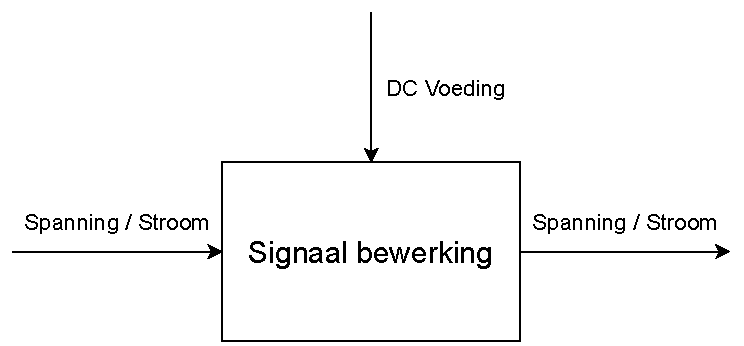
\includegraphics[width=0.45\linewidth]{pictures/Systeem_niveau_Systeemontwerp_Signaal_bewerking.drawio.pdf}
    \caption{Signaal bewerking subsysteem.}
    \label{fig:signaal_bewerking_subsysteem}
\end{figure}
\begin{table}[H]
    \centering
    \caption{Specificaties van Signaal bewerking subsysteem}
    \begin{tabular}{|c|c|}
        \hline
        \textbf{Module} & \textbf{Signaal bewerking} \\
        \hline
        \textbf{Ingangen} &  \begin{tabular}[c]{@{}c@{}}
        elektronische grootheid: ? \\
        DC-voeding \\
        \end{tabular} \\
        \hline
        \textbf{Uitgang(en)} & 
        Spanning / Stroom ? \\
        \hline
        \textbf{Functie} & \begin{tabular}[c]{@{}c@{}}
        Bewerkt het ingangssignaal van het subsysteem waar dit op is aangesloten\\
        en geeft dit op de uitgang bewerkt terug. \\
        De bewerking kan in het digitale of analoge domein gebeuren. \\
        \end{tabular} \\
        \hline
    \end{tabular}
    \label{tab:systeem_signaal_bewerking_sub_system}
\end{table}

Het vierde subsysteem is het Zend module subsysteem. Dit subsysteem is nodig om de informatie draadloos te versturen naar het basisstation waar alle informatie verzameld wordt. Om energie te besparen en niet constant data te versturen is het nodig dat dit subsysteem uitgezet kan worden. Dit is subsysteem is weergegeven in Figuur \ref{fig:zend_module_subsysteem} en Tabel \ref{tab:zend_module_subsysteem}.

\begin{figure}[H]
    \centering
    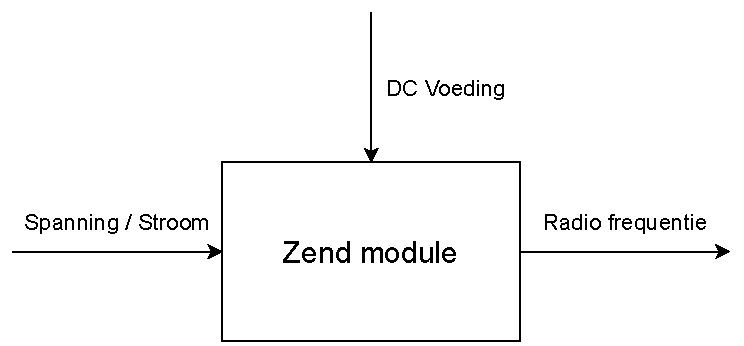
\includegraphics[width=0.45\linewidth]{pictures/Systeem_niveau_Systeemontwerp_Zend_module.drawio.pdf}
    \caption{Zend module subsysteem.}
    \label{fig:zend_module_subsysteem}
\end{figure}
\begin{table}[H]
    \centering
    \caption{Specificaties van Signaal bewerking subsysteem}
    \begin{tabular}{|c|c|}
        \hline
        \textbf{Module} & \textbf{Zend module} \\
        \hline
        \textbf{Ingangen} &  \begin{tabular}[c]{@{}c@{}}
        Spanning / Stroom ? \\
        DC-voeding \\
        \end{tabular} \\
        \hline
        \textbf{Uitgang(en)} & 
        Radio Frequentie waar de informatie over zonden wordt \\
        \hline
        \textbf{Functie} & \begin{tabular}[c]{@{}c@{}}
        Het ingangssignaal wordt omgezet naar een RF-signaal\\
        dit wordt gedaan om de informatie draadloos te versturen.\\
        \end{tabular} \\
        \hline
    \end{tabular}
    \label{tab:zend_module_subsysteem}
\end{table}

Het vijfde subsysteem is de ontvangst module. Dit subsysteem is nodig om de informatie van de zendmodule te ontvangen en te kunnen omvormen naar informatie die het basisstation kan begrijpen. Dit subsysteem is weergegeven in Figuur \ref{fig:ontvang_module_subsysteem} en Tabel \ref{tab:ontvang_module_subsysteem}.

\begin{figure}[H]
    \centering
    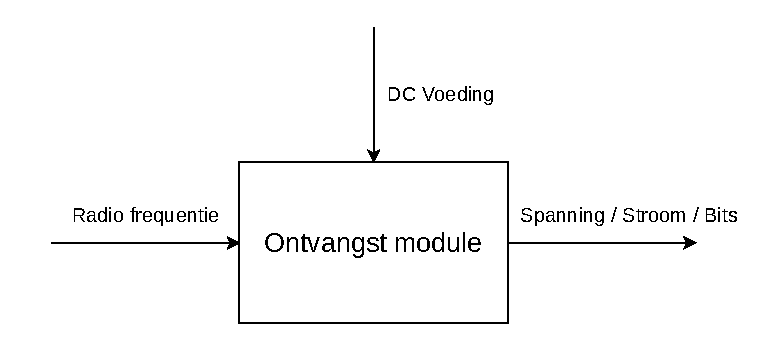
\includegraphics[width=0.45\linewidth]{pictures/Systeem_niveau_Systeemontwerp_Ontvang_module.drawio.pdf}
    \caption{Ontvangst module subsysteem.}
    \label{fig:ontvang_module_subsysteem}
\end{figure}
\begin{table}[H]
    \centering
    \caption{Specificaties van Signaal bewerking subsysteem}
    \begin{tabular}{|c|c|}
        \hline
        \textbf{Module} & \textbf{Ontvangst module} \\
        \hline
        \textbf{Ingangen} &  \begin{tabular}[c]{@{}c@{}}
        RF-signaal \\
        DC-voeding \\
        \end{tabular} \\
        \hline
        \textbf{Uitgang(en)} & 
        Spanning / Stroom / Bits ? \\
        \hline
        \textbf{Functie} & \begin{tabular}[c]{@{}c@{}}
        De RF-signalen op de ingang worden omgevormd naar een signaal \\
        wat het basis station kan begrijpen \\
        \end{tabular} \\
        \hline
    \end{tabular}
    \label{tab:ontvang_module_subsysteem}
\end{table}

Met deze vijf subsystemen is het mogelijk om ons systeem te ontwerpen. Elke van deze subsystemen heeft zijn eigen rol en kan meerdere keren voorkomen in het product.